\documentclass[twocolumn,a4paper]{article}

\usepackage[landscape,left=2cm,right=2cm,top=1cm,bottom=1cm]{geometry}

\fboxrule=0.75pt
\setlength{\fboxsep}{0pt}
\setlength{\columnsep}{25pt}

\pagenumbering{gobble}

\usepackage[T1]{fontenc}
\usepackage[utf8]{inputenc}
\usepackage[swedish]{babel}
\usepackage{csquotes}
\usepackage{hyperref}
\usepackage{url}
\usepackage{graphicx}
\usepackage[flushleft]{threeparttable}
\usepackage{booktabs}
\usepackage{amsmath}
\usepackage{amssymb}
\usepackage{caption}

\newcommand{\image}[1]{
\begin{figure}[ht]
	\centering
	\fbox{\resizebox{1\columnwidth}{!}{\includegraphics{#1}}}
\end{figure}
}


\begin{document}

%%%%%%%%%%%%%%%%%%%%%%%%%%%%%%%%%%%%%%%%%%%%%%%%%%%%%%%%%%%%%%%%%%%%%%%%%%%%%%%%%%%%%%%%%%%%%%%%%%%%%%%%%%%%%%%%%%%%%%%%%%%%%%%%%%%%%%%%%%%%
\section*{DNF solving}
You can use a truth table to solve DNF problems.
Start by adding a column for each literal with all combinations of 1s and 0s.
Then you add columns to your truth table for each subexpression until you've expressed the entire expression.
The rows containing a 1 in the final column are your answer.
See p.12 in Definitions för \emph{basic logic connectives}.
\begin{figure}[ht]
	\centering
	\fbox{\resizebox{0.85\columnwidth}{!}{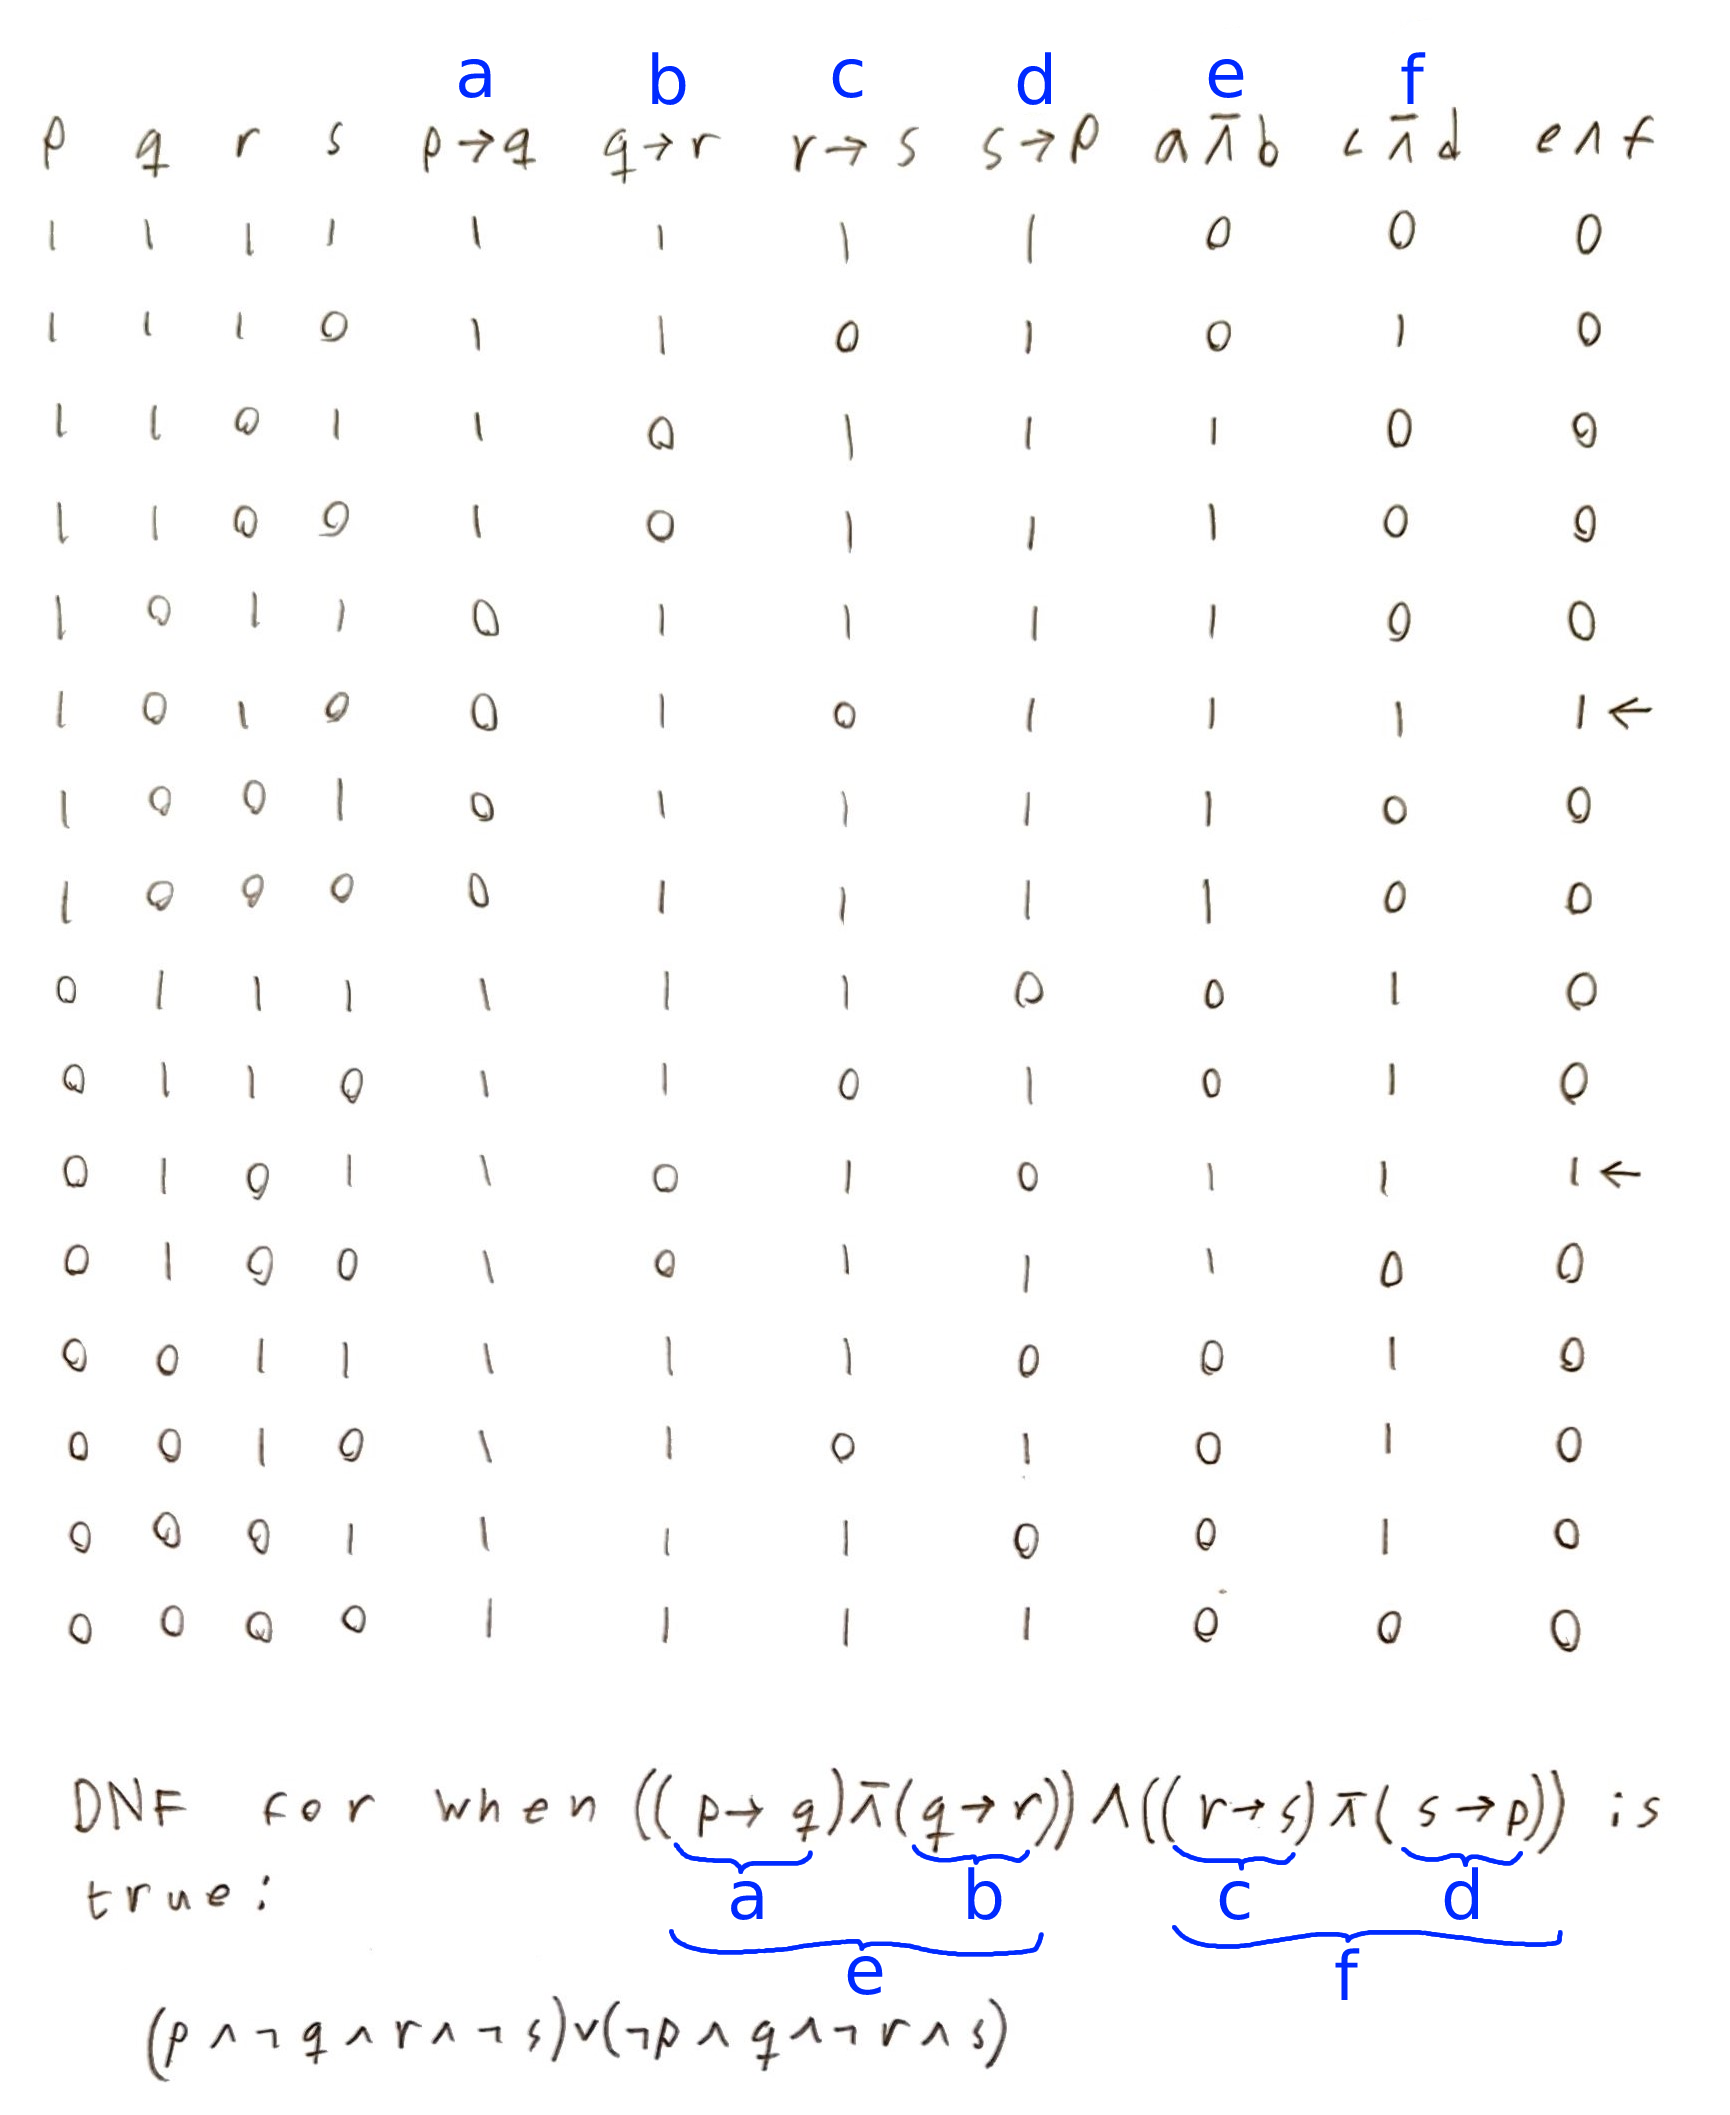
\includegraphics{2018_1/solution-5.1.png}}}
\end{figure}

%%%%%%%%%%%%%%%%%%%%%%%%%%%%%%%%%%%%%%%%%%%%%%%%%%%%%%%%%%%%%%%%%%%%%%%%%%%%%%%%%%%%%%%%%%%%%%%%%%%%%%%%%%%%%%%%%%%%%%%%%%%%%%%%%%%%%%%%%%%%
\newpage
\section*{Intervals}

Here is a question about understanding how intervals change when sending through functions and meet.

\begin{figure}[ht]
	\centering
	\vspace{-10pt}
	\fbox{\resizebox{0.85\columnwidth}{!}{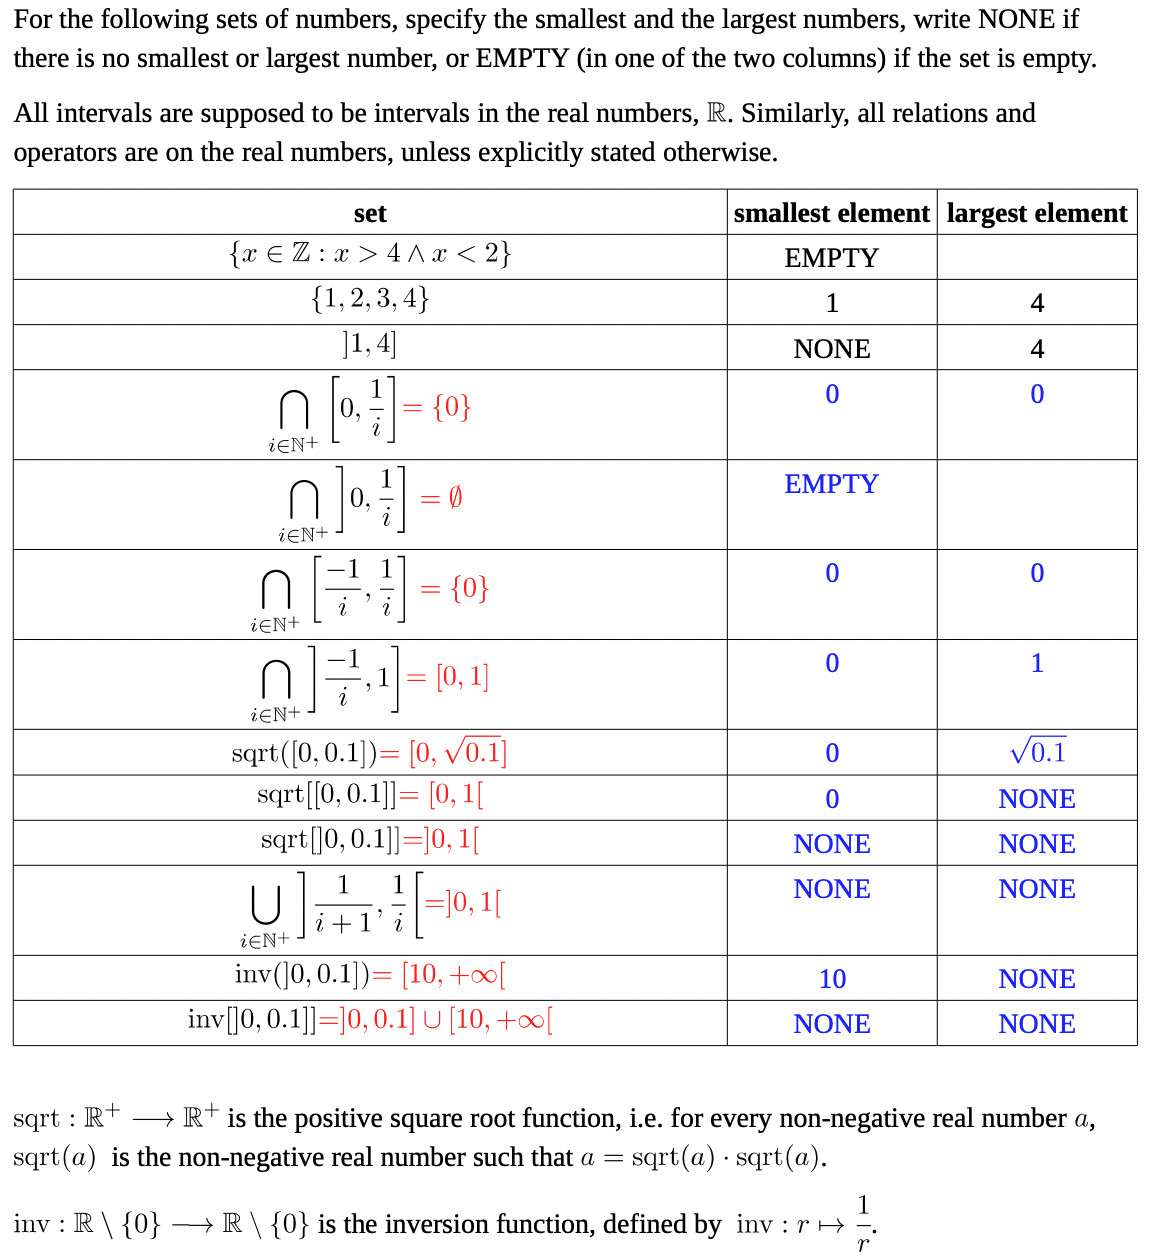
\includegraphics{2017_1/solution-1.png}}}
	\vspace{-10pt}
\end{figure}

Below is a explanation of how to think with intervals in more detail.
\begin{figure}[ht]
	\centering
	\vspace{-10pt}
	\fbox{\resizebox{0.85\columnwidth}{!}{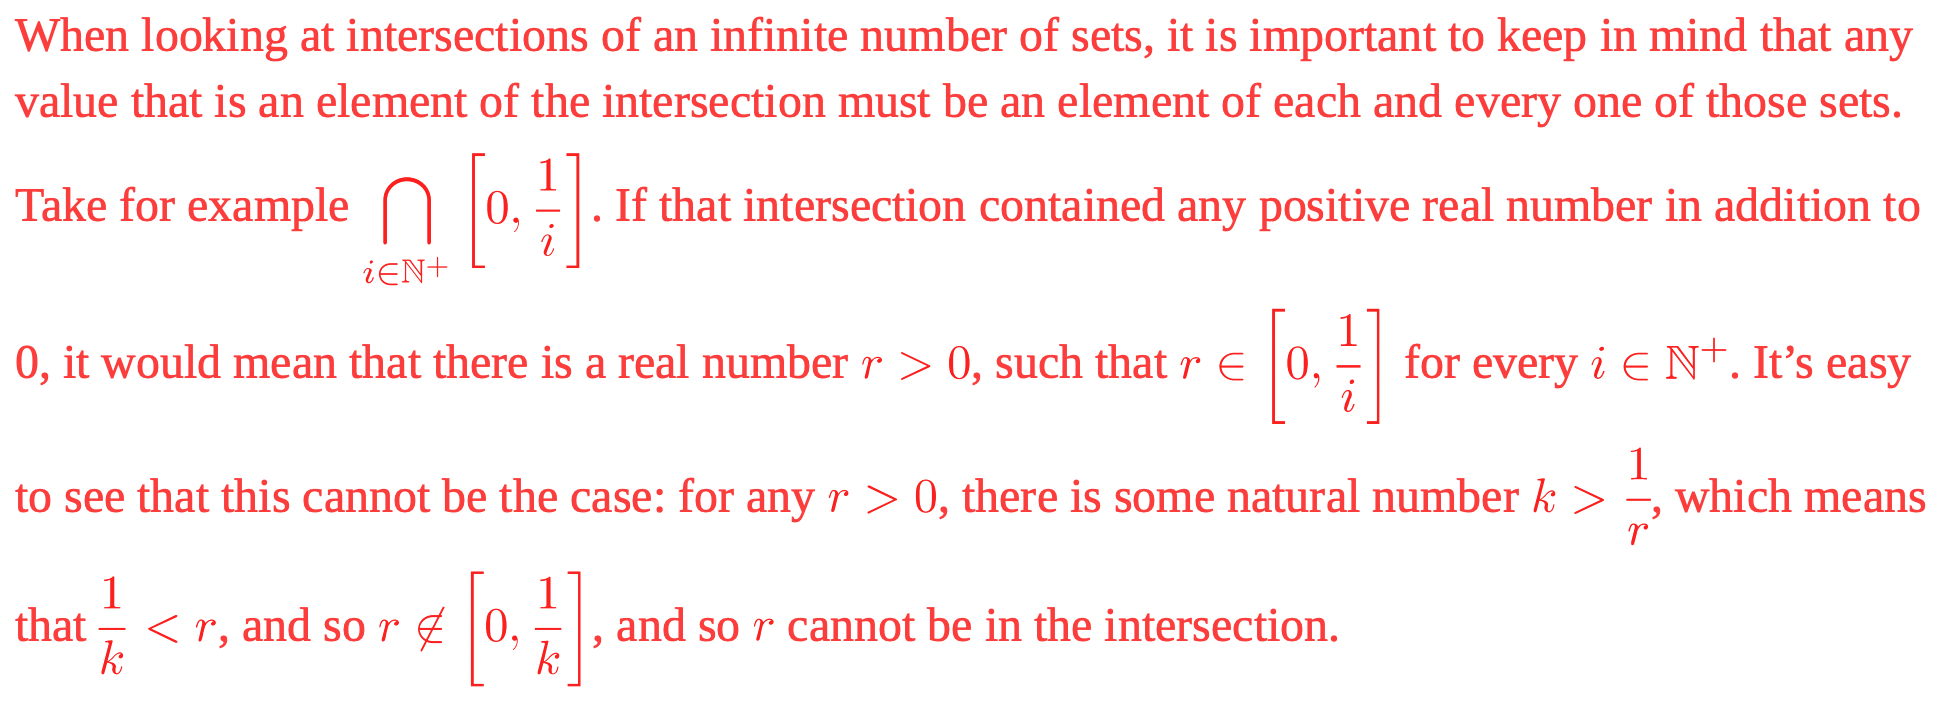
\includegraphics{2017_1/solution-1-explained.png}}}
	\vspace{-30pt}
\end{figure}

%%%%%%%%%%%%%%%%%%%%%%%%%%%%%%%%%%%%%%%%%%%%%%%%%%%%%%%%%%%%%%%%%%%%%%%%%%%%%%%%%%%%%%%%%%%%%%%%%%%%%%%%%%%%%%%%%%%%%%%%%%%%%%%%%%%%%%%%%%%%
\newpage
\section*{Injective and surjectiv}
This is a simpler example of injective and surjective functions.
The reason why this question is simpler is because we can define the domain and codomain separatly.

\begin{figure}[ht]
	\centering
	\fbox{\resizebox{0.95\columnwidth}{!}{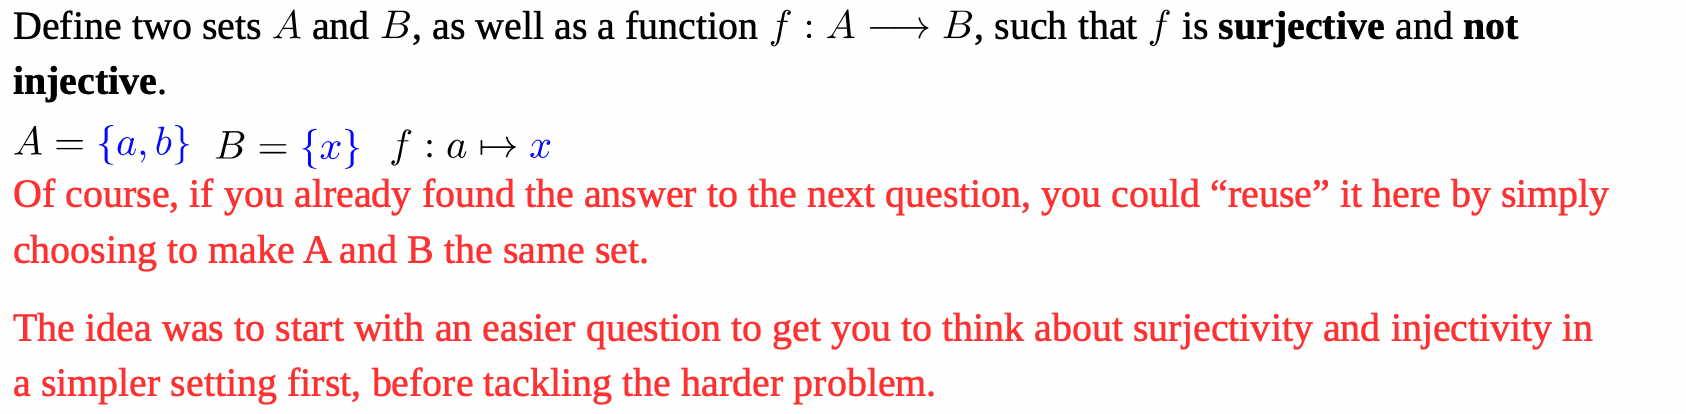
\includegraphics{2017_1/solution-2.png}}}
\end{figure}

When something should be surjective but \textbf{not} injective and the \(codomain = domain\) we need to utilize infinity.
Below, any element in the codomain could be reached from the domain by adding one to it.
Meaning it is surjective but we also point to the same element twice, 0 in this case.
\begin{figure}[ht]
	\centering
	\fbox{\resizebox{0.95\columnwidth}{!}{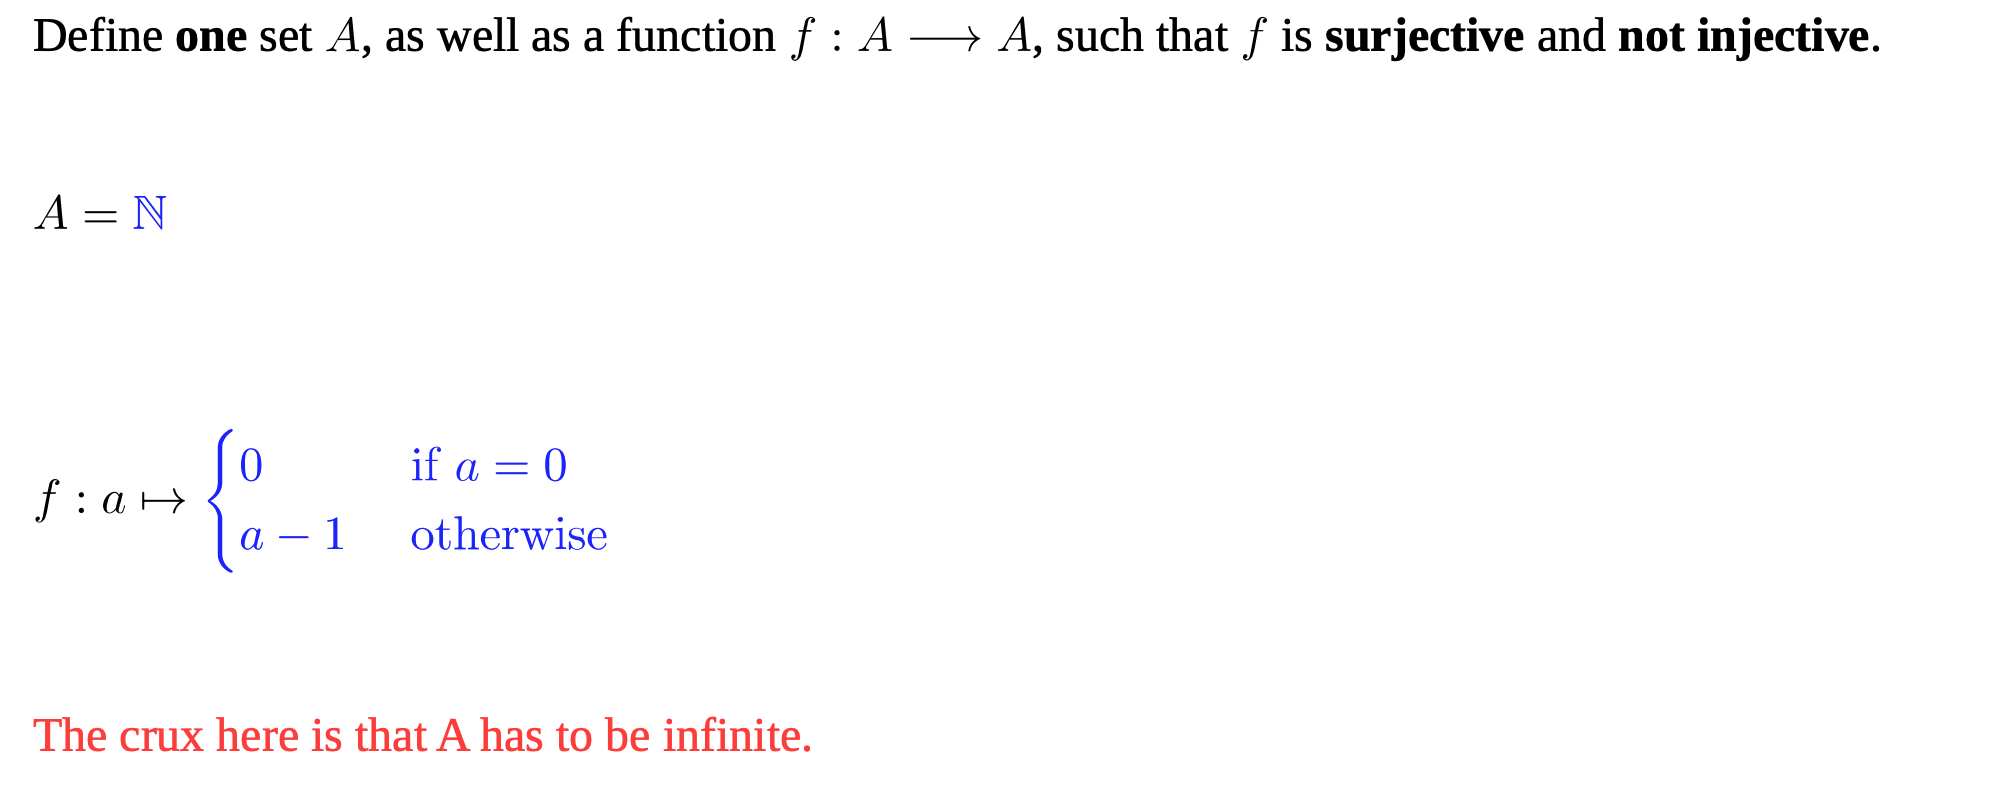
\includegraphics{2017_1/solution-3.png}}}
\end{figure}
\begin{figure}[ht]
	\centering
	\fbox{\resizebox{0.95\columnwidth}{!}{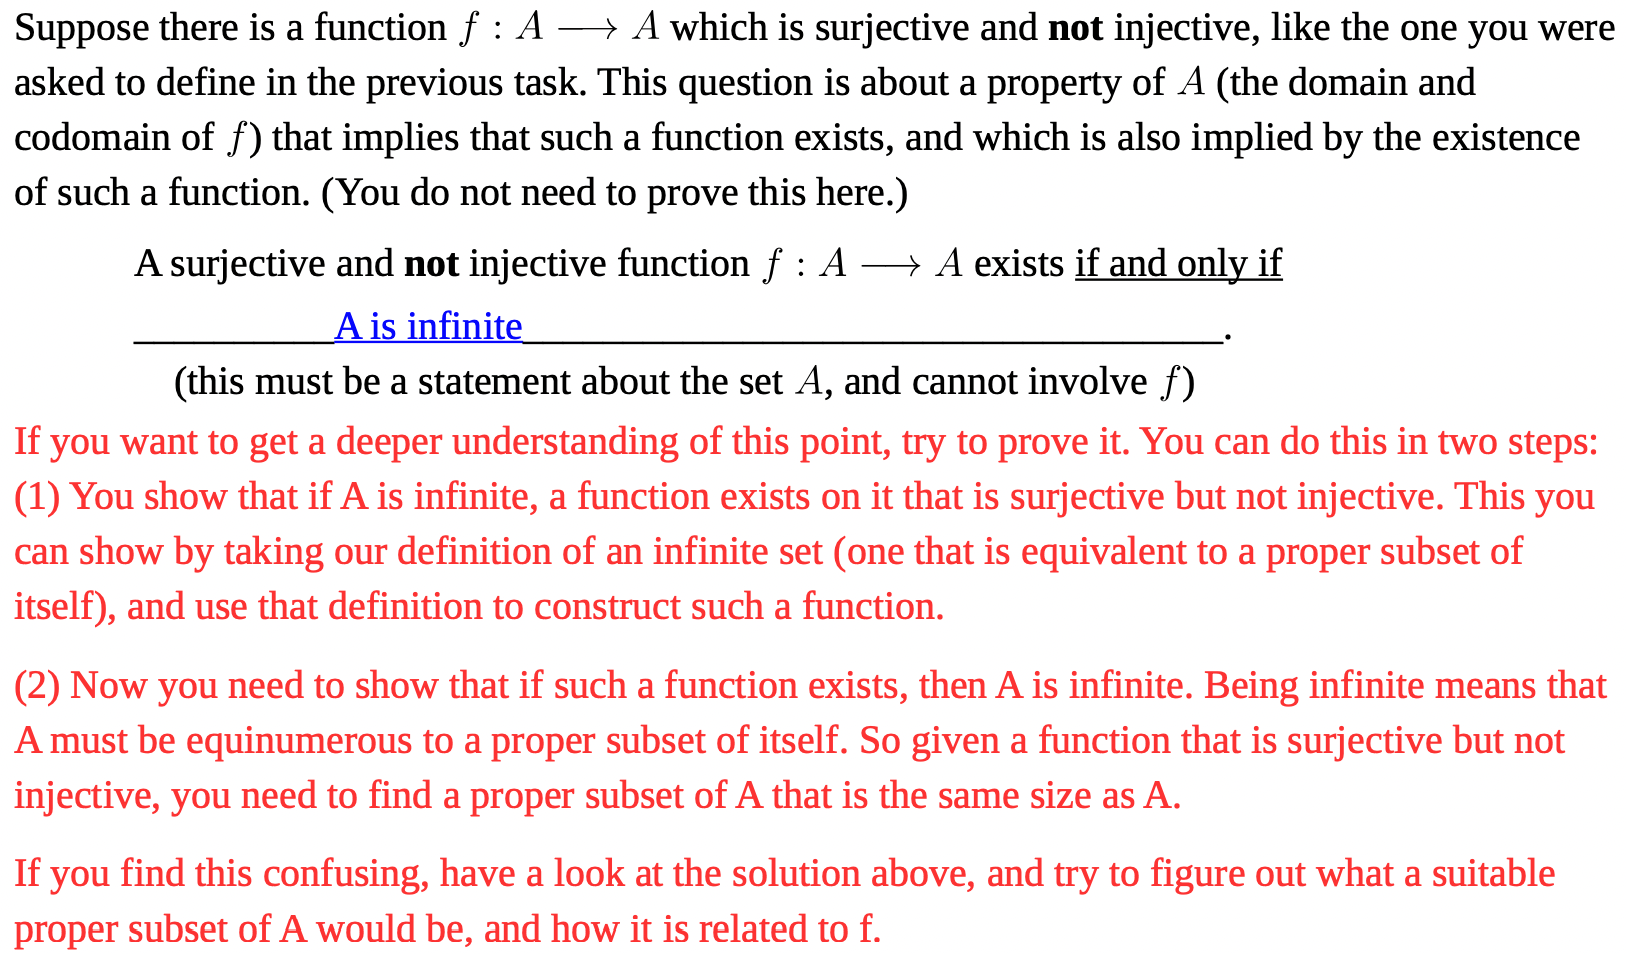
\includegraphics{2017_1/solution-4.png}}}
\end{figure}

%%%%%%%%%%%%%%%%%%%%%%%%%%%%%%%%%%%%%%%%%%%%%%%%%%%%%%%%%%%%%%%%%%%%%%%%%%%%%%%%%%%%%%%%%%%%%%%%%%%%%%%%%%%%%%%%%%%%%%%%%%%%%%%%%%%%%%%%%%%%
\newpage
\section*{Properties of paths, graphs and trees}
Properties of a \textbf{directed graph}, worth remembering is that no property is guaranteed.
We don't put any constraints on our graph meaning it could be any kind of relation,
for example every edge could be symmetric.
\begin{figure}[ht]
	\centering
	\fbox{\resizebox{0.95\columnwidth}{!}{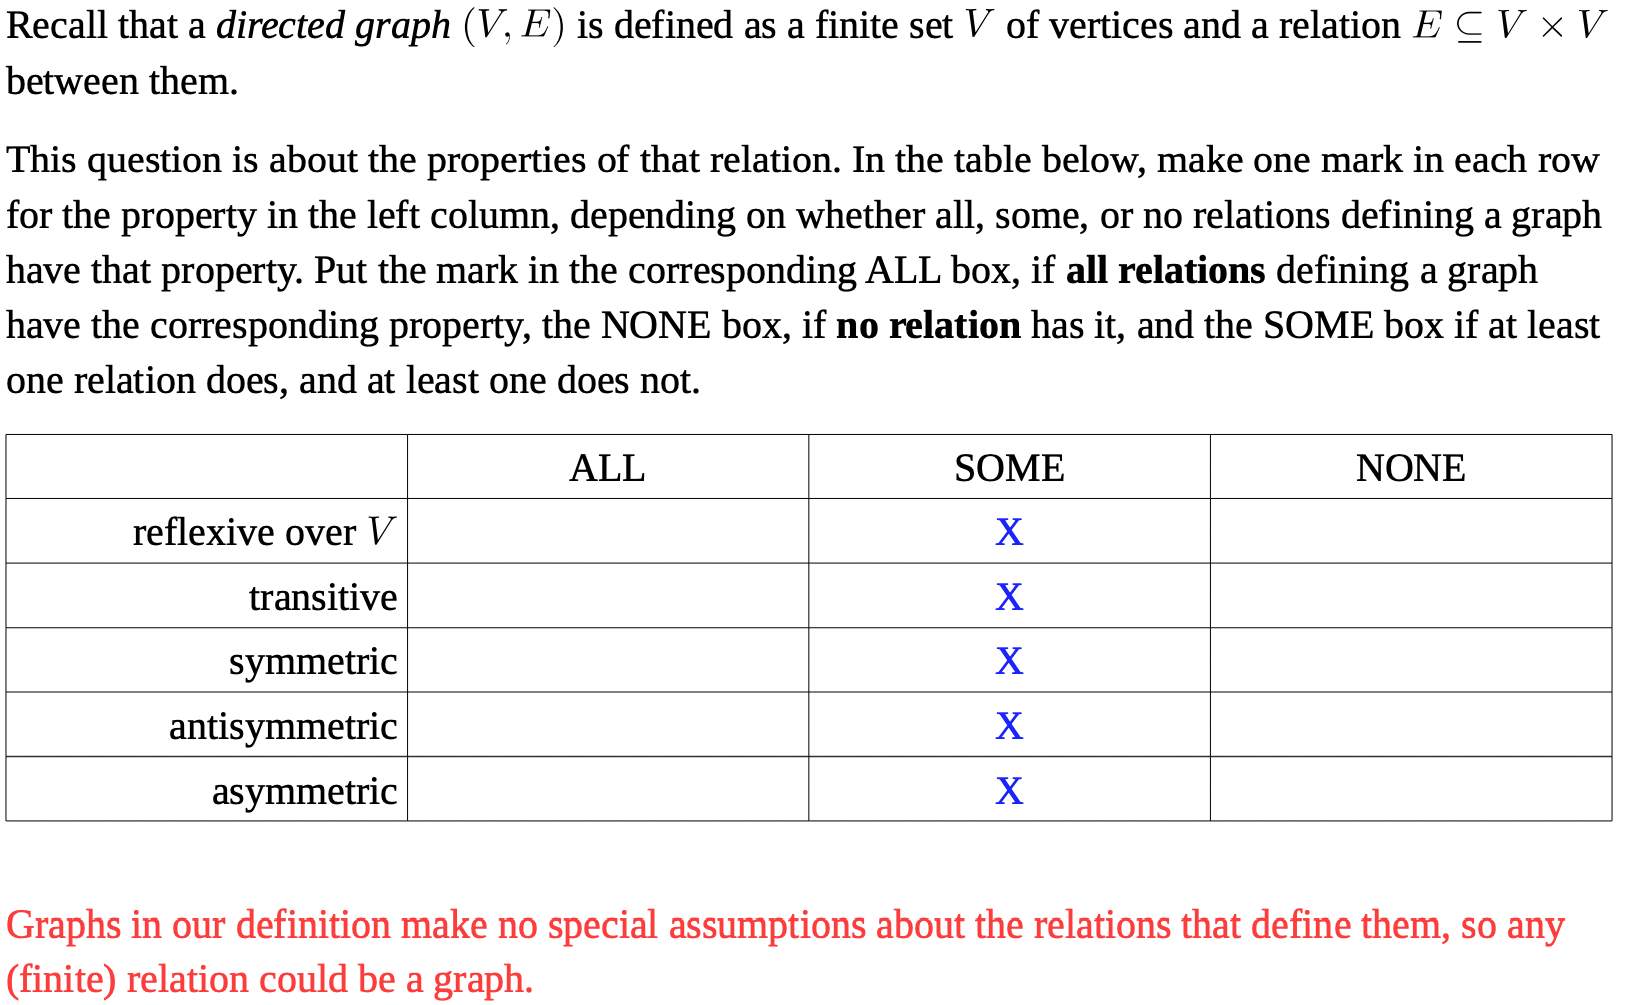
\includegraphics{2017_1/solution-5.png}}}
\end{figure}

Below are the properties of a \textbf{rooted tree}.
The reason it's antisymmetric and asymmetric is because if there exist (a,b) and (b,a) then there are multiple ways to reach b
(ie. \(a\rightarrow b\), \(a\rightarrow b\rightarrow a\rightarrow b\)).
The reason why it's antisymmetric is the same reason it is not reflexive.
\begin{figure}[ht]
	\centering
	\fbox{\resizebox{0.95\columnwidth}{!}{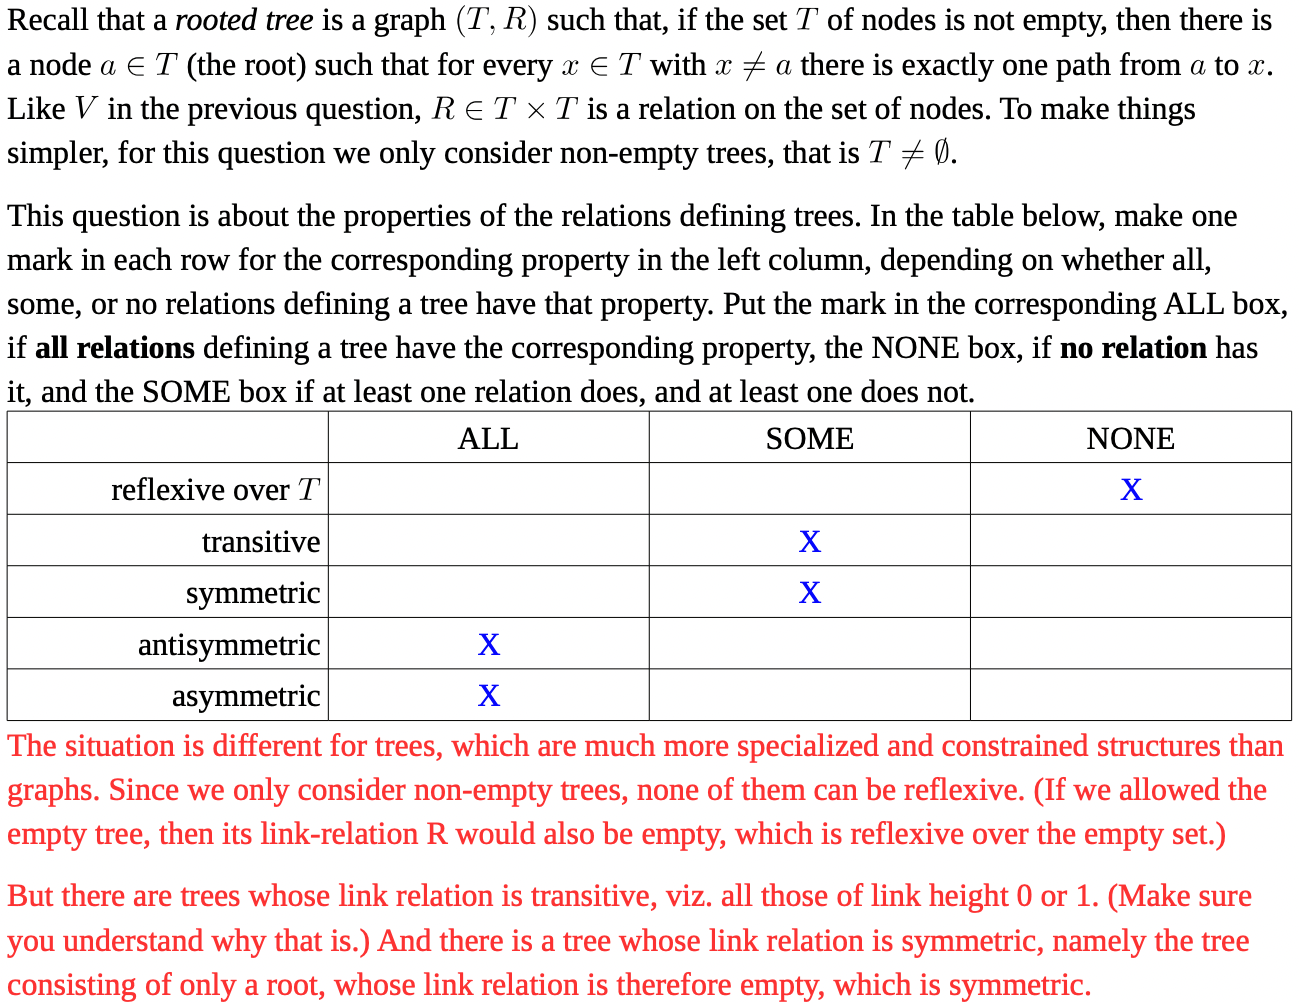
\includegraphics{2017_1/solution-6.png}}}
\end{figure}

%%%%%%%%%%%%%%%%%%%%%%%%%%%%%%%%%%%%%%%%%%%%%%%%%%%%%%%%%%%%%%%%%%%%%%%%%%%%%%%%%%%%%%%%%%%%%%%%%%%%%%%%%%%%%%%%%%%%%%%%%%%%%%%%%%%%%%%%%%%%
\newpage
\section*{Other important definitions}
\subsection*{Node height/depth}
The \textbf{link-height} (\emph{alias:} level) in a tree is defined recursively: that of the root is 0,
and that of each of the children of a node is one greater than that of the node.

The \textbf{node-height} (\emph{alias:} height) is defined by the same recursion,
except that the node-height of the root is set to 1.
Thus, for every node x, \(node-height(x) = link-height(x) + 1\).
As trees are usually drawn upside-down, the term `depth' is often used instead of `height'.

\subsection*{CNF}
Conjunctive normal form is like disjunctive normal form but `upside-down': the roles of disjunction and conjunction are reversed.
A basic disjunction is defined to be any disjunction of (one or more) literals in which no letter occurs more than once.
A formula is said to be in conjunctive normal form (CNF) iff it is a conjunction of (one or more) basic disjunctions

\subsection*{Edge cases for always/sometimes/never problems}
If you have a graph \((V, E)\), then you should check the edge cases where:
\begin{enumerate}
	\item \(V=\emptyset \) or \(E=\emptyset \).
	\item \(V\) only contains 1 node or 2 nodes.
	\item \(E\) contains a connection in one direction but not back. And when it contains a connection in both directions.
	\item All nodes are connected to all nodes.
\end{enumerate}

\subsection*{Quantifiers}

\(\forall x\in\emptyset(\ldots) = true\). \\
\(\exists x\in\emptyset(\ldots) = false\).

\subsection*{Logic operators}
\begin{enumerate}
	\item $\alpha \barwedge \beta = \neg (\alpha \wedge \beta)$ and $\neg \alpha = (\alpha \barwedge \alpha)$
\end{enumerate}

\subsection*{Image of n-ary}
When computing the image, we treat the last element of a tuple as the `output'.
\begin{equation}
	R(a_1, \ldots, a_{n-1}) = \{a \in A : (a_1, \ldots, a_{n-1}, a) \in R \}
\end{equation}

\newpage
\subsection*{Extras}

\image{2017_1/2017a/uppg3.png}
\image{2017_1/2017a/uppg5.png}
\image{2017_1/2017a/uppg4-no-crop.png}
\image{2017_1/2017a/4-help.png}
\image{misc/2018-2-2-q.png}
\image{misc/2018-2-2-s.png}
\image{misc/vertecies-uppg.png}
\image{misc/vertecies-sol.png}
\image{misc/languages.png}
\image{misc/5-1.png}
\image{misc/5-2.png}


\end{document}

